\documentclass{resume}

\begin{document}

\fontfamily{ppl}\selectfont

\noindent
\begin{tabularx}{\linewidth}{@{}m{0.8\textwidth} m{0.2\textwidth}@{}}
{
    \Large{Rubén Tobar Nicolau} \newline
    \small{
        \clink{
            \href{mailto:rubentobarnicolau@gmail.com}{rubentobarnicolau@gmail.com} 
            \textbf{·} 
            {\fontdimen2\font=0.75ex 677 11 91 39}
%            \textbf{·}
%            \href{https://www.rubtobar.com}{rubtobar.com}
            
            \href{https://www.linkedin.com/in/rubtobar/}{linkedin.com/in/rubtobar/}
            \textbf{·} 
    		\href{https://github.com/rubtobar}{github.com/rubtobar}
    	} \newline
        Madrid, España
    }
} & 
{
    \hfill
    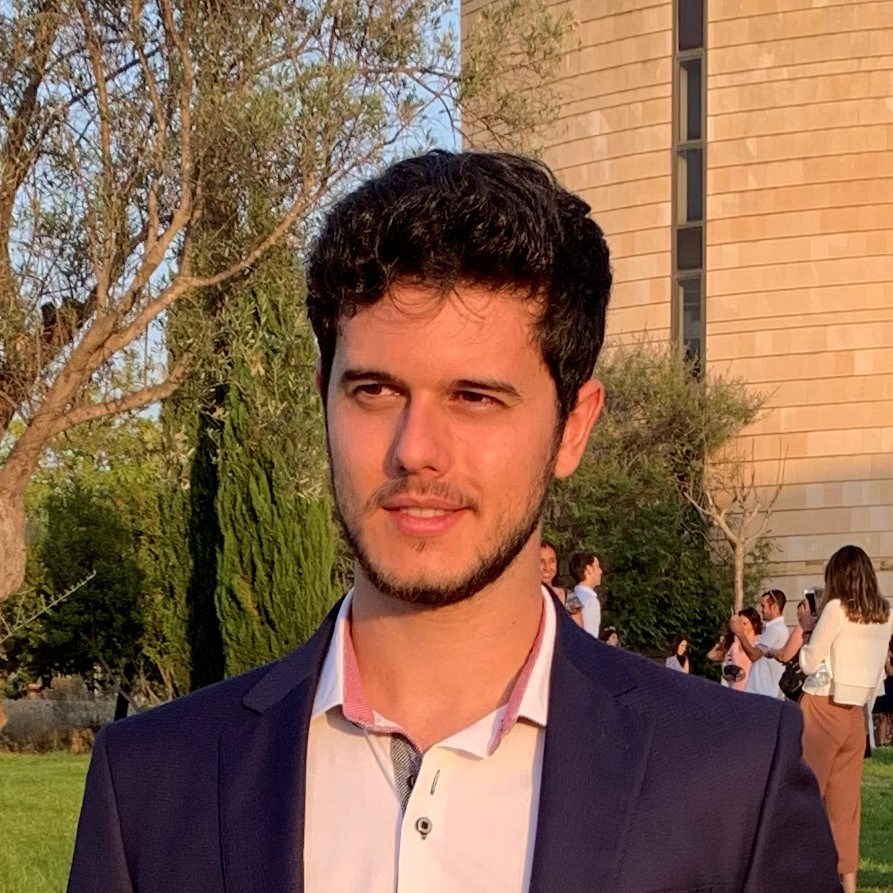
\includegraphics[width=2.8cm]{images/me.jpg}
}
\end{tabularx}

\begin{center}
\begin{tabularx}{\linewidth}{@{}*{2}{X}@{}}
% left side %
{
    \csection{Experiencia}{\small
        \begin{itemize}
            % item 1 %
			\item 
			\textbf{Ingeniería de Sistemas para la Defensa de España} \newline
			Ingeniero de sistemas y ciberseguridad
			\begin{itemize}
				\item Administración de sistemas
				\item Ciberseguridad
				\item Explotación de datos
				\item Formación continua
			\end{itemize}
			\begin{footnotesize}
			\textit{marzo 2020 - Actualidad}
			\end{footnotesize}
			
            % item 2 %
            \item 
            \textbf{Juniper Innovating Travel Technology} \newline
            Ingeniero de software
            \begin{itemize}
            	\item Empresa con alcance mundial. 
            	\item Obtención de requisitos de software.
            	\item .NET framework
            	\item Booking engine
            \end{itemize}
            \begin{footnotesize}
            	\textit julio 2017 - octubre 2017
            \end{footnotesize}
            
            
        \end{itemize}
    
    }
    \csection{Formación}{\small
        \begin{itemize}
            % item 1 %
            \item \frcontent{Máster universitario en Inteligencia Artificial}{Universidad Internacional de La Rioja}{}{En curso}
            % item 2 %
            \item \frcontent{Grado en Ingeniería Informática}{Universidad de las Islas Baleares}{}{2019}
            % item 3 %
            \item \frcontent{Beca ERASMUS+ Bolonia, Italia}{Alma Mater Studiorum Università di Bologna}{}{2017}
        \end{itemize}
    }
    \csection{Otros datos}{\small
        \begin{itemize}
        	% item 1 %
        	\item \textbf{Idiomas} \newline Español y Catalán (Nativo), Inglés (Alto)
        	\footnotesize
        \end{itemize}
    }
} 
% end left side %
& 
% right side %
{
    \csection{Tecnologías}{\small
        \begin{AutoMultiColItemize}
			\item Java
			\item Python
			\item C++
			\item C\#
			\item C
			\item JavaScript
			\item TensorFlow
			\item Kubernetes
			\item Angular
			\item Flutter
			\item Dockers
			\item .NET
			\item Bash
        \end{AutoMultiColItemize}
    }
    \csection{Proyectos}{\small
        \begin{itemize}
            \item \frcontent{Compilador \newline \clink{
            		\href
            		{https://github.com/rubtobar/compiler}
            		{\footnotesize [github.com/rubtobar/compiler]}}}
            	{Compilador de lenguaje tipo java a código ensamblador}{}{Java, Assebly Code, Regex, LARL Parser Generator.}
            \item \frcontent{Filtros Morfológicos \newline \clink{
            		\href{https://github.com/rubtobar/filtros-morfologicos}
            		{\footnotesize[github.com/rubtobar/filtros-morfologicos]}}}
            	{Eliminación de ruido impulsivo en imágenes binarias de huellas dactilares.}{}{Python, Jupyter Notebook, OpenCV}
            \item \frcontent{Modelo Vista Controlador \newline 
            \clink{
            	\href{https://github.com/rubtobar/MVC}
            	{\footnotesize[github.com/rubtobar/MVC]}}}
            {Sistema de gestión reservas de hoteles utilizando BBDD relacional, MVC y Razor.}{}{C\#, .NET 5.0, Razor, SQL Database}
            \item \frcontent{Sistema de ficheros \newline 
            \clink{
            	\href{https://github.com/rubtobar/file-system}
            	{\footnotesize[github.com/rubtobar/file-system]}}}
        {Sistema de ficheros con semáforos MUTEX para concurrencia.}{}{C, Make, Linux, Shell}
        \end{itemize}
    }
    \csection{Intereses \& Hobbies }{\small
        \vspace{0.32cm}
        \begin{tabularx}{\linewidth}{@{}*{4}{>{\centering\arraybackslash}X}@{}}
            {\centering
            
\includegraphics[width=0.8cm]{images/sports.png}
            } &
            {\centering
            
\includegraphics[width=0.8cm]{images/camera.png}
            } & 
            {\centering
            
\includegraphics[width=0.8cm]{images/guitar.png}
            } &
            {\centering
            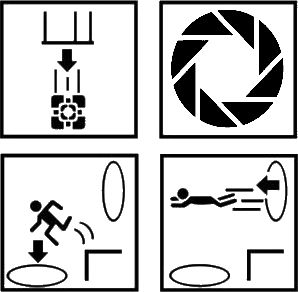
\includegraphics[width=0.8cm]{images/aperture.png}
            } \\
            {\footnotesize Deporte} & {\footnotesize Fotografía} & {\footnotesize Guitarra} & {\footnotesize Nuevas tecnologías}
        \end{tabularx}
    }
}
\end{tabularx}
\end{center}
\end{document}